% Figure of the starter paper (scripts/gen-starters.ts compiles it to templates/starters/paper/figures/convergence.pdf).
\documentclass[border=2pt]{standalone}
\usepackage[T1]{fontenc}
\usepackage{lmodern}
\usepackage{amsmath}
\usepackage{pgfplots}
\pgfplotsset{compat=1.18}
\begin{document}
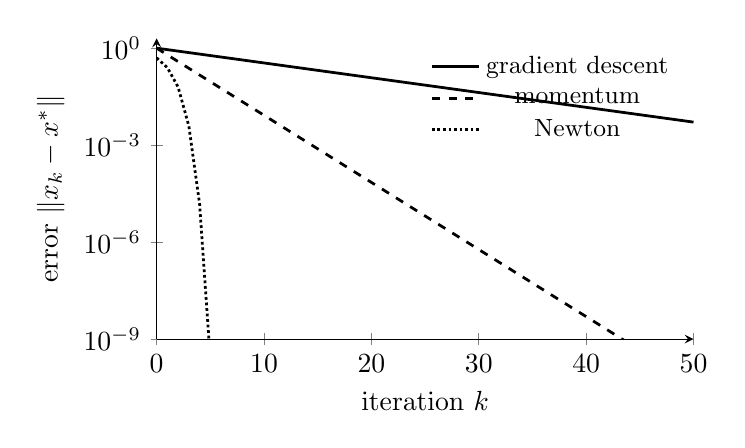
\begin{tikzpicture}
\begin{axis}[width=8.4cm, height=5.4cm, ymode=log, xmin=0, xmax=50, ymin=1e-9, ymax=2,
  xlabel={iteration $k$}, ylabel={error $\lVert x_k-x^\ast\rVert$}, axis lines=left,
  legend style={draw=none, font=\small, fill=none, at={(0.98,0.98)}, anchor=north east},
  every axis plot/.append style={line width=1pt, samples=51, domain=0:50}]
\addplot[black] {0.9^x};
\addplot[black, dashed] {0.62^x};
\addplot[black, densely dotted, domain=0:7, samples=8] {0.5^(2^x)};
\legend{gradient descent, momentum, Newton}
\end{axis}
\end{tikzpicture}
\end{document}
